\documentclass[sigplan,anonymous,review,10pt]{acmart}
\usepackage{subcaption}
\usepackage{algorithm}
\usepackage{algpseudocode}
\usepackage{makecell}

\AtBeginDocument{%
  \providecommand\BibTeX{{%
    Bib\TeX}}}

\acmConference[Conf. '26]{Anonymous Conference}{2026}{City, Country}
% CRUCIAL for EuroSys review phase
\setcopyright{none}

% TODO: whether to remove these
\renewcommand\footnotetextcopyrightpermission[1]{} %remove copyright 
\settopmatter{printacmref=false} %remove ACM reference format

% %% Rights management information.  This information is sent to you
% %% when you complete the rights form.  These commands have SAMPLE
% %% values in them; it is your responsibility as an author to replace
% %% the commands and values with those provided to you when you
% %% complete the rights form.
% \setcopyright{acmlicensed}
% \copyrightyear{2018}
% \acmYear{202}
% \acmDOI{XXXXXXX.XXXXXXX}
% %% These commands are for a PROCEEDINGS abstract or paper.
% \acmConference[Conference acronym 'XX]{Make sure to enter the correct
%   conference title from your rights confirmation email}{June 03--05,
%   2018}{Woodstock, NY}
% %%
% %%  Uncomment \acmBooktitle if the title of the proceedings is different
% %%  from ``Proceedings of ...''!
% %%
% %%\acmBooktitle{Woodstock '18: ACM Symposium on Neural Gaze Detection,
% %%  June 03--05, 2018, Woodstock, NY}
% \acmISBN{978-1-4503-XXXX-X/2018/06}


%%
%% Submission ID.
%% Use this when submitting an article to a sponsored event. You'll
%% receive a unique submission ID from the organizers
%% of the event, and this ID should be used as the parameter to this command.
\acmSubmissionID{146}

%%
%% For managing citations, it is recommended to use bibliography
%% files in BibTeX format.
%%
%% You can then either use BibTeX with the ACM-Reference-Format style,
%% or BibLaTeX with the acmnumeric or acmauthoryear sytles, that include
%% support for advanced citation of software artefact from the
%% biblatex-software package, also separately available on CTAN.
%%
%% Look at the sample-*-biblatex.tex files for templates showcasing
%% the biblatex styles.
%%

%%
%% The majority of ACM publications use numbered citations and
%% references.  The command \citestyle{authoryear} switches to the
%% "author year" style.
%%
%% If you are preparing content for an event
%% sponsored by ACM SIGGRAPH, you must use the "author year" style of
%% citations and references.
%% Uncommenting
%% the next command will enable that style.
%%\citestyle{acmauthoryear}


%%
%% end of the preamble, start of the body of the document source.
\begin{document}

%%
%% The "title" command has an optional parameter,
%% allowing the author to define a "short title" to be used in page headers.
\title{CoLoRA: Execution-First Miss Recovery for Multi-LoRA MoE Decode Serving}


\author{Anonymous Submission}

%%
%% By default, the full list of authors will be used in the page
%% headers. Often, this list is too long, and will overlap
%% other information printed in the page headers. This command allows
%% the author to define a more concise list
%% of authors' names for this purpose.
% \renewcommand{\shortauthors}{Trovato et al.}

%%
%% The abstract is a short summary of the work to be presented in the
%% article.
\begin{abstract}
Multi-LoRA MoE decode serving creates a new memory-management regime for LLM inference. Once tenant-specific LoRA modules are attached to sparsely activated expert layers, the effective unit of access and reuse becomes a joint expert--LoRA object rather than an expert or adapter alone. Our analysis shows that this shift breaks conventional cache locality assumptions: hot-set concentration collapses, cache scaling exhibits sharply diminishing returns, and the remaining performance loss moves into the latency tail.

We present CoLoRA, a multi-LoRA MoE serving runtime that treats GPU-cold misses as an execution-first recovery problem rather than a promotion-first caching problem. CoLoRA adopts a residency-aware hot/cold dual-path design: GPU-resident objects execute on the hot path, while GPU-cold objects trigger a CPU cold path that computes only the LoRA residual from host-resident weights and merges it back for the current token. CoLoRA further incorporates deferred promotion and selective temporal predispatch to improve future reuse and partially overlap cold-path latency. By decoupling cold-object execution from GPU residency management, CoLoRA avoids pipeline stalls during cache misses while preserving efficient GPU execution for hot objects and base-model computation. Compared with promotion-first multi-LoRA serving baselines, CoLoRA reduces P99 Time-Per-Output-Token (TPOT) by up to 44\% while maintaining high throughput.
\end{abstract}

%%
%% The code below is generated by the tool at http://dl.acm.org/ccs.cfm.
%% Please copy and paste the code instead of the example below.
%%
%\begin{CCSXML}
%<ccs2012>
%   <concept>
%       <concept_id>10010520.10010521.10010542.10010546</concept_id>
%       <concept_desc>Computer systems organization~Heterogeneous (hybrid) systems</concept_desc>
%       <concept_significance>500</concept_significance>
%       </concept>
%   <concept>
%       <concept_id>10011007.10010940.10010941.10010949.10010950</concept_id>
%       <concept_desc>Software and its engineering~Memory management</concept_desc>
%       <concept_significance>500</concept_significance>
%       </concept>
%   <concept>
%       <concept_id>10011007.10010940.10010941.10010949.10010957.10010688</concept_id>
%       <concept_desc>Software and its engineering~Scheduling</concept_desc>
%       <concept_significance>500</concept_significance>
%       </concept>
% </ccs2012>
%\end{CCSXML}

%\ccsdesc[500]{Computer systems organization~Heterogeneous (hybrid) systems}
%\ccsdesc[500]{Software and its engineering~Memory management}
%\ccsdesc[500]{Software and its engineering~Scheduling}

%%
%% Keywords.
% Note: CCS Concepts and user-defined keywords are required for all articles over two pages in length. (https://www.acm.org/publications/authors/submissions)
% \keywords{Multi-LoRA Serving, Heterogeneous Execution}


% \received{20 February 2007}
% \received[revised]{12 March 2009}
% \received[accepted]{5 June 2009}

%%
%% This command processes the author and affiliation and title
%% information and builds the first part of the formatted document.
\maketitle

\section{Introduction}
\label{sec:introduction}

Large-scale LLM serving is increasingly shaped by the convergence of two trends: MoE base models~\cite{jiang2024mixtral} and LoRA-based multi-tenant adaptation~\cite{hu2022lora,sheng2024slora}. In practice, these trends meet in \emph{multi-LoRA MoE serving}. While existing multi-LoRA systems target dense modules such as attention layers and shared FFNs, they do not address adaptation on sparsely activated MoE expert layers~\cite{chen2024punica,sheng2024slora}. This gap is critical: MoE expert FFN blocks comprise the majority of model capacity, making them the natural target for tenant-specific specialization~\cite{fedus2022switch,schulman2025lora}. This combination couples the compute efficiency of MoE with the parameter efficiency of LoRA. However, it creates a new serving regime in which request-time sparse routing and tenant-specific adapter selection jointly shape the active weights. This significantly enlarges and diversifies the inference working set, rendering it difficult to manage with existing caching strategies.
% v2: Large-scale LLM serving is increasingly shaped by the convergence of two trends that are individually effective but jointly nontrivial to serve: sparse Mixture-of-Experts (MoE) base models~\cite{jiang2024mixtral} and LoRA-based multi-tenant adaptation~\cite{hu2022lora,sheng2024slora}. In practice, these trends naturally meet in \emph{multi-LoRA MoE serving}. Existing multi-LoRA serving systems, however, are primarily designed for dense backbones and do not directly address adaptation on sparsely activated MoE expert layers~\cite{chen2024punica,sheng2024slora}. Such adaptation is both natural and important: MoE expert FFN blocks comprise a large fraction of model capacity and are a natural target for tenant-specific specialization~\cite{fedus2022switch, schulman2025lora}. The resulting combination is attractive because it couples the compute efficiency of MoE with the parameter efficiency of LoRA. At the same time, it creates a new serving regime in which request-time sparse routing and tenant-specific adapter selection jointly shape the active weight set, making the inference working set larger, more diverse, and harder to manage efficiently.
%
%Note: In this version, \cite{gale2023megablocks} to be moved to Related Work if not cited elsewhere.
%
% v1: Large-scale LLM serving is increasingly shaped by the convergence of two trends that are each effective in isolation but jointly challenging in deployment: sparse Mixture-of-Experts (MoE) base models~\cite{jiang2024mixtral} and LoRA-based multi-tenant adaptation~\cite{hu2022lora,sheng2024slora}. In production settings, these trends naturally meet in \emph{multi-LoRA MoE serving}. While LoRA is widely used as a lightweight mechanism for tenant-specific customization, existing multi-LoRA serving systems have largely been designed for dense-model adaptation rather than expert-layer adaptation in sparse MoE models~\cite{chen2024punica,sheng2024slora}. Extending LoRA to MoE expert layers is both natural and practically important, because expert FFN blocks account for a large fraction of model capacity and provide a high-leverage target for task- or tenant-specific specialization~\cite{fedus2022switch, schulman2025lora}. This combination is appealing from a deployment perspective: MoE reduces base-model compute, while LoRA enables efficient per-tenant customization without replicating the full model. However, it also creates a distinct serving regime in which dynamic sparse routing~\cite{gale2023megablocks} and long-tailed multi-tenant adaptation~\cite{} jointly determine which expert- and adapter-side weights are needed for each request, increasing access diversity and complicating locality management during inference.

This enlarged and more diverse working set becomes especially problematic during \emph{decode} in prefill--decode deployments~\cite{agrawal2023sarathi,patel2024splitwise}. Unlike prefill, which can often amortize weight-loading costs across many prompt tokens, decode operates under tight inter-token latency SLOs: generation is highly memory-bandwidth bound, and any weight miss on the critical path directly translates to pipeline stalls and ITL degradation. Consequently, the granularity of weight management becomes critical: in pure MoE serving, the natural unit is the expert; in conventional multi-LoRA serving, it is the adapter, and prior systems such as S-LoRA~\cite{sheng2024slora} and VaLoRA~\cite{mi2025empower} therefore adopt adapter-centric designs that assume dense adapter loading.

In multi-LoRA MoE decode, however, a request only needs the LoRA residuals for the selected experts, so the effective unit of access and reuse is neither an expert alone nor an adapter alone, but a joint expert--LoRA object. These objects are larger than the attention-side LoRA units emphasized in prior systems, because expert-layer LoRA scales with the wide FFN dimensions rather than the narrower attention projections~\cite{shazeer2017outrageously}. At the same time, the base MoE model already occupies most device memory, leaving only limited residual VRAM for caching such objects~\cite{zhu2024deepseek}. The result is a larger and more fragmented working set that breaks the locality assumptions of prior caches and makes decode latency increasingly unpredictable.

To quantify this locality regime, we conduct a trace-driven study using Alibaba LoRA serving traces augmented with realistic MoE expert routing patterns~\cite{lin2025understanding}. The study shows that once access is modeled at the granularity of joint expert--LoRA objects, the hot set becomes far less concentrated. Under a 2K-object cache budget, expert-only modeling covers 98.4\% of accesses, while realistic joint-object modeling covers only 21.8\% and 13.9\% under correlated (C2) and independent (C1) adapter--expert assignment, respectively (Figure~\ref{fig:motivation-breakdown}(a)). As a result, cache scaling becomes markedly less effective: expert-only modeling reaches its target P99 TPOT with a small cache, whereas realistic joint-object workloads still fail to reach that same target even with much larger capacity (Figure~\ref{fig:motivation-breakdown}(b)). Under practical budgets, the penalty appears mainly in the tail rather than the median: median TPOT remains near 1.2\,ms, while P99 TPOT rises to 6.70\,ms, a 5.6$\times$ slowdown (Figure~\ref{fig:motivation-breakdown}(c)). Together, these results show that in multi-LoRA MoE decode, GPU-cold misses are not transient anomalies removable through modest cache growth; they are persistent tail events on the decode critical path.

Once accesses to GPU-non-resident expert--LoRA objects become unavoidable, the central problem shifts from \emph{how to avoid misses} to \emph{how to serve them on the decode critical path}. Existing GPU-centric systems typically handle such misses with a promotion-first policy: required weights are first promoted from host memory to GPU memory, and execution resumes only after that promotion completes~\cite{sheng2023flexgen}. This works when misses are infrequent and future reuse is sufficient to amortize migration cost. In multi-LoRA MoE decode, however, a miss may correspond to only a small amount of LoRA-side computation for a single token, with limited computation to amortize PCIe transfer latency and no guarantee of near-term reuse. In this regime, promotion-first recovery becomes a blocking synchronization point that directly stalls token generation. The resulting systems question is therefore: when a joint expert--LoRA object is not resident on the GPU, should the current token stall for synchronous promotion, or should the miss be served through a different execution path?

We design CoLoRA, a decode-time runtime for multi-LoRA MoE serving that replaces blocking promotion-first recovery with execution-first miss recovery. CoLoRA uses a residency-aware hot/cold dual-path design for expert--LoRA computation during decode. GPU-resident objects remain on the hot path, while GPU-cold objects are handled through a separate cold path rather than triggering immediate synchronous promotion. Crucially, CoLoRA does not offload the full expert computation to the CPU. Instead, it exploits a decode-time data-movement asymmetry: servicing a cold LoRA residual requires exchanging only per-token activation vectors, whereas promotion-first recovery must first transfer the full expert--LoRA weight object to the GPU. The base MoE expert computation therefore remains on the GPU, while the corresponding cold LoRA residual is computed on the CPU from host-resident weights and merged back for the current token. In this way, CoLoRA turns GPU-cold misses from unconditional migration barriers into bounded execution events on the decode critical path.

CoLoRA is built on three key ideas. (1) Execution-first residency-aware hot/cold serving: GPU-resident expert--LoRA objects remain on the hot path, while GPU-cold objects are handled through a separate miss path instead of immediate blocking promotion. (2) Decoupled miss-recovery scheduling through a CPU cold path: when an object is GPU-cold, CoLoRA computes only the corresponding LoRA residual via a bounded CPU-side recovery path, keeping the GPU as the primary engine for hot objects and base-model expert computation. (3) Locality-driven background optimization: deferred promotion and selective temporal predispatch improve reuse under fragmented access patterns and overlap cold-path data movement with later hot-path decode steps, ensuring demand execution remains decoupled from prediction accuracy or synchronous migration.

Our contributions are threefold:
\begin{itemize}
    \item We identify and characterize a decode-time GPU-cold-miss regime in multi-LoRA MoE serving. Using trace-driven analysis, we show that when joint expert--LoRA objects become the unit of access, locality deteriorates structurally: hot-set concentration weakens, cache scaling shows diminishing returns, and performance loss shifts into the latency tail. 
    %We identify and characterize a new decode-time GPU-cold-miss regime in multi-LoRA MoE serving. Using trace-driven analysis, we show that when joint expert--LoRA objects become the effective unit of access, locality deteriorates structurally: hot-set concentration weakens, cache scaling yields sharply diminishing returns, and the remaining performance loss shifts into the latency tail.

    \item We show that, in this regime, miss recovery should be treated as an execution problem rather than only a caching problem. We formulate the decode-time cost asymmetry between promotion-first recovery and execution-first recovery, and show why serving the current token need not require immediate restoration of full GPU residency.

    \item We design CoLoRA, a decode-time serving runtime that realizes this execution-first principle through three coordinated mechanisms: a residency-aware hot/cold dual-path architecture, a decoupled miss-recovery scheduler, and locality-driven background optimizations for future reuse.

\end{itemize}

We implement CoLoRA in a multi-LoRA MoE serving prototype ..... . Compared with representative multi-LoRA serving baselines ......, CoLoRA reduces P99 TPOT by up to 1.8$\times$ while maintaining comparable throughput by ....., showing that execution-first recovery improves tail robustness without sacrificing efficient GPU execution.  

%We demonstrate that CoLoRA makes multi-LoRA MoE decode serving more resilient under realistic cache pressure by removing blocking promotion from the critical path of GPU-cold misses, preserving the GPU as the primary engine for hot objects and base-model execution, and reducing tail-latency inflation.

\begin{figure*}[t]
    \centering

    \begin{minipage}{0.31\textwidth}
        \centering
        \small\textbf{(a) Locality breaks under joint objects}
        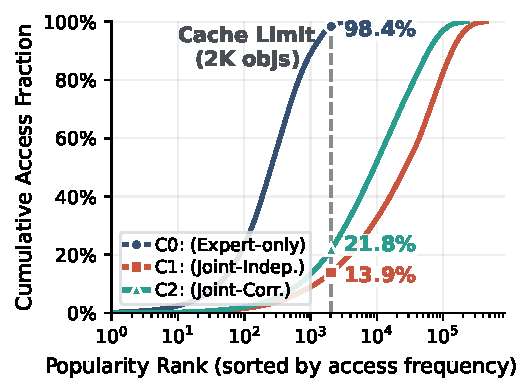
\includegraphics[width=\linewidth]{figures/motivation/motivation_panel_a_root_cause.pdf}
    \end{minipage}\hfill
    \begin{minipage}{0.31\textwidth}
        \centering
        \small\textbf{(b) Cache scaling loses effectiveness}
        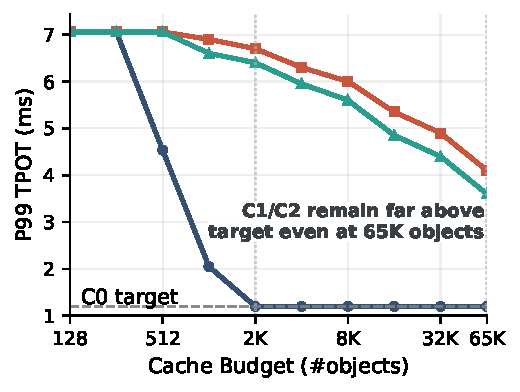
\includegraphics[width=\linewidth]{figures/motivation/motivation_panel_b_capacity_illusion.pdf}
    \end{minipage}\hfill
    \begin{minipage}{0.31\textwidth}
        \centering
        \small\textbf{(c) Tail latency explodes under misses}
        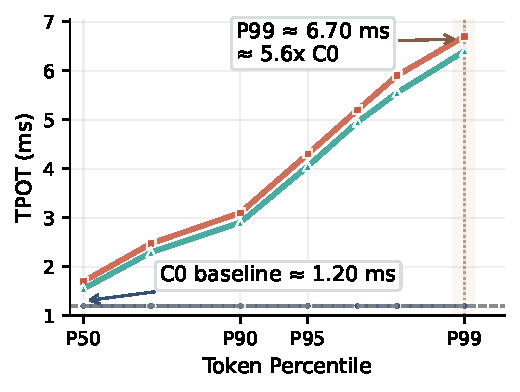
\includegraphics[width=\linewidth]{figures/motivation/motivation_panel_c_tail_blowout_budget_2048.pdf}
    \end{minipage}

    \caption{
    \textbf{Why caching alone is insufficient for multi-LoRA MoE decode serving.}    
 \textbf{Why caching alone is insufficient for multi-LoRA MoE decode serving.}
(a) Once the cache object becomes a joint expert--LoRA object, access concentration drops sharply.
(b) This locality loss makes cache scaling much less effective: expert-only modeling reaches the target P99 TPOT with a small cache, whereas joint-object workloads remain far above the same target even at much larger capacity.
(c) Under a practical cache budget, the penalty appears mainly in the tail rather than the median.
Together, these results show that the main challenge is not raw cache capacity, but how GPU-cold misses are handled on the decode critical path.
}    
    \label{fig:motivation-breakdown}
\end{figure*}


\section{Background, Motivation, and Challenges}
\label{sec:background}

\subsection{Background: Expert--LoRA Computation}
\label{subsec:background}

In multi-LoRA MoE serving, decode-time execution combines two request-dependent effects. For each generated token, the shared MoE base model routes computation to a small subset of experts, while each request carries its own tenant- or task-specific LoRA adaptation. As a result, decode depends on both routed expert weights and the corresponding LoRA states for the active request, creating a fine-grained, highly variable access pattern on the per-token critical path.
This pattern changes the natural unit for reasoning about locality and misses. In dense multi-LoRA serving, adapter-level reasoning is often sufficient because accesses tend to concentrate on one adapter's weights. In MoE decode, however, LoRA computation is needed only for the experts selected for the current token. The relevant access unit is therefore neither an expert alone nor an adapter alone, but their joint use in decode, which we call an \emph{expert--LoRA joint object}.

This matters most during decode. Unlike prefill, decode operates with small effective batch sizes, repeats routing and weight-access decisions once per token, and exposes miss-handling overheads directly in token latency. As a result, when expert--LoRA joint objects cannot be kept within practical GPU cache budgets, the challenge is not only how to manage GPU residency, but also how to recover GPU-cold misses without inflating per-token latency.

\subsection{Motivation: Joint Objects Reshape Locality}
\label{subsec:motivation}

\subsubsection{Joint Objects as the Decode Access Unit.}
\label{subsec:joint-object}

A central question is what abstraction the system should use to reason about locality, residency, and misses.

In sparse MoE decode, each token activates only a small subset of experts. When multiple LoRA adapters coexist, accesses no longer concentrate on entire adapters or on experts alone, but on the LoRA states associated with the routed experts for the current request. The effective unit of access and reuse is therefore the expert--LoRA joint object.

Reasoning at coarser granularity obscures this access pattern. Adapter-level management is too coarse because it groups many expert slices together with the few actually needed for the current token. Expert-level management is incomplete in multi-tenant serving because it ignores adapter identity: although the routed expert set may repeat across requests, the associated LoRA adapters vary across tenants, so collapsing accesses by expert alone systematically overestimates reuse. To understand the systems consequences of this shift in access granularity, we next compare decode locality and runtime behavior under expert-only and expert--LoRA joint-object views.

\subsubsection{Joint Objects Weaken Decode Locality.}
\label{subsec:case-study}

To examine whether this finer-grained access view matters in practice, we conduct a trace-driven case study under three workload conditions. \texttt{C0} uses expert-only keys. 
\texttt{C1} uses expert--LoRA joint keys under independent assignment, where adapter identity is sampled independently of expert routing. \texttt{C2} uses the same joint keys under correlated assignment, where certain adapters are more likely to co-occur with specific experts. This setup separates the effect of finer-grained keying itself from the extent to which structured adapter--expert affinity can partially preserve locality. We use Alibaba LoRA serving traces~\cite{lin2025understanding} to model request arrivals and LoRA invocations, and replay the resulting decode access streams under these three conditions. As illustrated inFigure~\ref{fig:motivation-breakdown}, modeling accesses as joint expert--LoRA objects triggers a cascade of locality and performance degradations.

%As illustrated in Figure \ref{fig:motivation-breakdown}, modeling accesses as joint objects triggers a cascade of system-level degradations, demonstrating that traditional caching strategies are insufficient for this workload.

\noindent {\bf Locality weakens under joint objects.}
Moving from coarse-grained to joint-object modeling substantially fragments decode locality. Figure~\ref{fig:motivation-breakdown}(a) shows that the access distribution flattens once expert routing and adapter identity are modeled jointly. Because accesses are spread across a combinatorial space of expert--LoRA pairs, the hot set becomes markedly less dominant. As a result, a practical GPU cache captures a smaller fraction of total accesses, increasing reuse distances and making cold starts more frequent.

\noindent {\bf Cache scaling loses effectiveness.}
Because locality is fundamentally weakened, simply increasing GPU cache capacity no longer resolves the problem. Figure~\ref{fig:motivation-breakdown}(b) shows that the expert-only layout reaches its target P99 TPOT with only 2K cached objects, whereas the joint-object layouts remain substantially above the same target across the entire cache sweep and still fail to recover it even at 65K cached objects. The issue is therefore not merely insufficient cache capacity. Once access granularity fragments locality, scaling cache size yields sharply diminishing returns. In practice, systems must operate under constrained budgets where cold misses remain unavoidable.

\noindent {\bf Tail latency explodes under misses.}
The most severe consequence of this locality fragmentation appears in decode latency. Figure~\ref{fig:motivation-breakdown}(c) evaluates TPOT under a practical GPU cache budget. While median TPOT remains near-optimal at approximately 1.2\,ms, the degradation is concentrated in the tail: P99 latency increases by roughly 5.6$\times$. Because decode repeats routing and parameter-access decisions token by token, cold misses stall the synchronous execution path and disproportionately penalize requests that traverse uncached expert--LoRA intersections.

Taken together, these results sharpen the systems bottleneck in multi-LoRA MoE decode. Once expert--LoRA joint objects become the effective unit of access, the core issue is no longer only whether locality can be preserved, but whether inevitable cold misses can be served without directly inflating token latency. This shifts attention from locality alone to the feasibility of alternative miss-handling strategies on the decode critical path.

\subsubsection{Why Execution-First Recovery Can Be Viable.}
\label{subsec:feasibility}
The case study results show that, under practical GPU cache budgets, cold misses remain persistent once expert--LoRA joint objects become the effective unit of access. The next question is therefore not only how to enlarge the hot set, but whether miss handling can be restructured to better match decode-time constraints. Decode is favorable to this restructuring: execution advances token by token, per-adapter batches are small, and misses across requests are often only partially synchronized. As a result, a miss need not be treated as a global stall; part of its recovery work may be isolated and overlapped.

\begin{figure}[t]
  \centering
  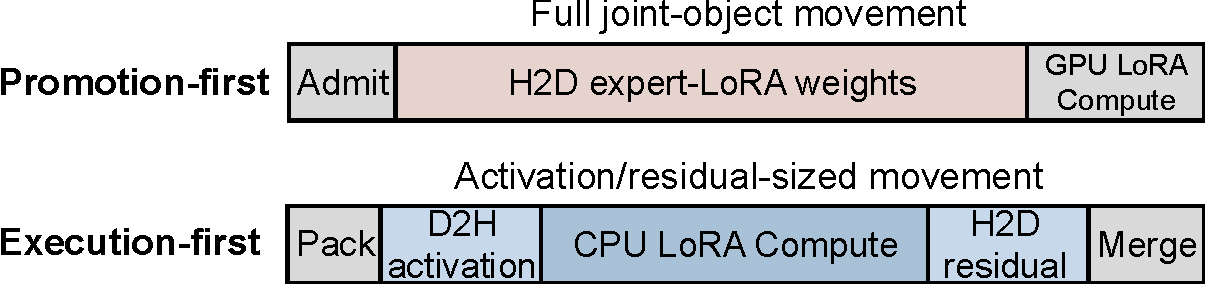
\includegraphics[width=\linewidth]{figures/miss_cost_compare.pdf}
  \caption{
     \textbf{Promotion-first vs. execution-first synchronous miss cost.}
      Promotion-first places full weight migration on the current token's critical path. Execution-first instead exchanges activation/residual-sized state, computes only the missing LoRA contribution on the CPU, and merges it back. The key distinction is the synchronous payload on the decode critical path.
  }
  \label{fig:miss-cost-compare}
\end{figure}

A key observation is that a decode-time GPU-cold miss creates an asymmetry between restoring residency and serving the current token, as illustrated in Figure~\ref{fig:miss-cost-compare}. Under a promotion-first policy, the system must first move the missing expert--LoRA object into GPU memory and only then resume execution. For the current token, however, what is immediately required is not residency restoration itself, but completion of the missing expert--LoRA contribution for the routed expert. This distinction matters because expert-layer LoRA objects are relatively large, whereas the per-token activation state for the current decode step is comparatively small. Promotion-first recovery therefore places a large weight transfer on the current token's critical path.

This asymmetry suggests that feasibility should be judged by how much miss-recovery work must remain on the current token's critical path, not by whether CPU execution is universally faster than GPU execution. If the missing LoRA contribution can be computed by exchanging activation-sized state while leaving base expert computation on the GPU, then a cold miss need not be treated as an unconditional residency-restoration barrier. Instead, it can be handled as a bounded execution event whose visible cost depends on available overlap with other ready GPU work.

This perspective is especially relevant in multi-tenant MoE decode, where mixed hit/miss batches are common and misses are not perfectly synchronized across requests. In such settings, forcing every cold object through immediate promotion risks turning a per-request miss into a broader stall that delays unrelated ready work. By contrast, an execution-first design can isolate recovery to the faulting request while allowing other ready requests to continue on the GPU.

This does not imply that execution-first recovery is always preferable. When adapter diversity is low, the effective working set fits comfortably in GPU memory, or near-term reuse is strong enough to amortize immediate promotion, a promotion-first policy becomes more competitive. We therefore target the regime identified in Figure~\ref{fig:motivation-breakdown}: cache-pressured multi-LoRA MoE decode, where joint-object locality is structurally fragmented, cold misses remain unavoidable, and miss recovery should be optimized for exposed latency rather than immediate residency restoration.

\subsection{Design Goal and Challenges}
\label{subsec:challenges}

The results above show that once expert--LoRA joint objects become the effective unit of access, practical GPU cache capacity alone can no longer eliminate cold misses. In multi-LoRA MoE decode, cold misses therefore become persistent events on the critical path rather than rare outliers. This shifts the central question from how to avoid every miss to how to recover unavoidable misses without inflating per-token latency. These observations imply one core design goal and two resulting challenges.

%The results above reveal a shift in the role of caching for multi-LoRA MoE decode serving. Once expert--LoRA joint objects become the effective unit of access, locality weakens enough that cold misses cannot be eliminated through practical GPU cache capacity alone. Cold misses are therefore no longer rare outliers absorbed by a sufficiently large hot set. Instead, they become persistent events on the decode critical path, shifting the central question from how to avoid every miss to how to recover unavoidable misses without inflating per-token latency. These observations therefore imply one core design goal and two resulting challenges.

\noindent {\bf Goal: Serve at expert--LoRA granularity under expanded and fragmented working sets.}
Under joint-object modeling, the effective key space expands substantially, while reuse becomes weaker and more fragmented across requests. Adapter-level management is too coarse because it retains many expert slices that are never touched, whereas expert-only reasoning overestimates reuse by ignoring adapter diversity. The runtime must operate at expert--LoRA granularity, matching actual computation without assuming that caching alone can absorb the working-set expansion.
%Under joint-object modeling, the effective key space expands substantially, while reuse becomes weaker and more fragmented across requests. This makes coarse-grained management ineffective: adapter-level residency retains many expert slices that are never touched, whereas expert-only reasoning overestimates reuse by ignoring adapter diversity. At the same time, naive fine-grained residency increases fragmentation pressure on the hot set and makes limited GPU capacity more vulnerable to transient cold objects. The runtime must therefore serve at expert--LoRA granularity, which matches actual computation, without assuming that caching alone can absorb the resulting working-set expansion.

\noindent {\bf Challenge 1: Recovering cold misses without promotion-first stalls on decode.}
\label{subsec:challenge-miss}
In this regime, many misses correspond to objects whose near-term reuse is too weak to justify immediate promotion. A conventional promotion-first policy therefore turns each miss into a blocking recovery event on the current token. The runtime must instead support completion of the current expert--LoRA computation without making immediate GPU promotion the only recovery path, while still preserving the option to promote later when reuse warrants it.
%In this regime, many misses correspond to objects whose near-term reuse is too weak to justify immediate promotion. If the system continues to use a conventional promotion-first policy, each such miss becomes a blocking recovery event: the current token must wait for weight migration before expert--LoRA computation can proceed. Under decode-time latency sensitivity, this directly amplifies tail latency. The runtime therefore needs a different default recovery strategy for cold misses. Instead of forcing all misses through immediate GPU promotion, it must support completion of the current expert--LoRA computation without making promotion the only recovery path, while still preserving the option to promote objects later when future reuse warrants it.

\noindent {\bf Challenge 2: Making cold-path recovery practical under decode constraints.}
\label{subsec:challenge-overlap}
Changing the recovery abstraction is not sufficient by itself. If cold-path execution is too slow or poorly integrated with the decode pipeline, it merely replaces GPU promotion stalls with CPU-side stalls or new queueing behavior. The runtime must therefore make cold-path recovery efficient under small, irregular decode batches and preserve overlap with GPU hot-path or base-model computation whenever dependencies allow.
%Changing the miss-recovery abstraction is not sufficient by itself. If cold-path execution is too slow, the system merely replaces GPU promotion stalls with CPU-side stalls. If it is poorly integrated with the decode pipeline, heterogeneous execution introduces new queueing and tail behavior rather than alleviating the original bottleneck. The runtime must therefore make cold-path recovery efficient enough to operate under small, irregular decode batch sizes, and organize execution to preserve overlap between cold-miss handling and GPU hot-path or base-model computation whenever dependencies allow. The challenge is not only to provide an alternative recovery path, but to ensure that this path reduces exposed miss latency rather than becoming a new bottleneck.

Together, these observations motivate CoLoRA's design: a runtime that operates at expert--LoRA granularity, replaces promotion-first recovery with an execution-first path, and organizes cold-path handling to preserve overlap and limit exposed decode latency.
%Together, these observations motivate CoLoRA's design: a runtime that operates at expert--LoRA granularity, replaces promotion-first miss recovery with an execution-first path, and organizes cold-path handling to preserve overlap and limit exposed decode latency.


\section{CoLoRA Design}
\label{sec:design}

\subsection{Overview}
\label{subsec:design-overview}

\begin{figure}[t]
    \centering
    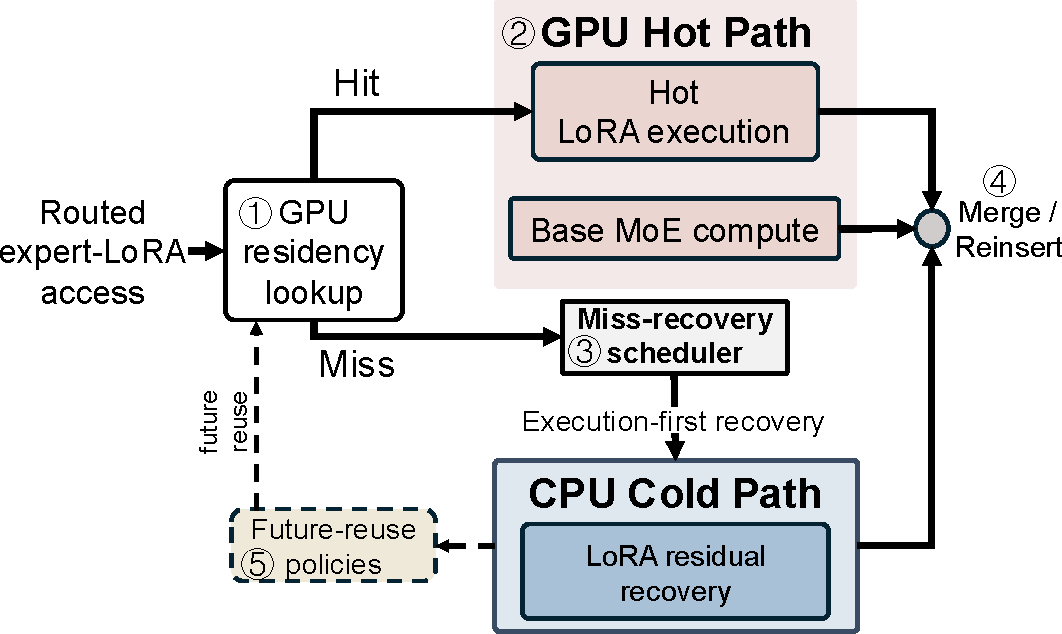
\includegraphics[width=\columnwidth]{figures/architecture.pdf}
    \caption{
    \textbf{CoLoRA overview.}
    For each routed expert--LoRA access, CoLoRA checks GPU residency at joint-object granularity. Hits execute on the GPU hot path together with base MoE computation. Misses are handled by the miss-recovery scheduler and served through a CPU cold path that computes the missing LoRA residual before merging it back into the decode stream. Future-reuse policies update residency for later accesses off the current-token critical path.
    }
    \label{fig:colora-overview}
\end{figure}


CoLoRA realizes this design through an execution-first runtime for cache-pressured multi-LoRA MoE decode. It uses expert--LoRA joint objects as the uniform unit of runtime control---covering residency lookup, miss recovery, admission, and background optimization---while separating current-token recovery from future-reuse optimization.%Its key objective is therefore to ensure that an unavoidable miss does not become a synchronization point for unrelated ready work.

Figure~\ref{fig:colora-overview} shows the overall design. On each routed access, GPU-resident objects execute on the GPU hot path. GPU-cold objects are recovered through a CPU cold path that computes the missing LoRA residual for the current token, rather than forcing synchronous promotion of the full object.

CoLoRA organizes these responsibilities into two coupled loops. The foreground loop serves the current token: residency lookup sends hits to GPU hot-path LoRA execution and misses to CPU cold-path residual recovery; completed residuals are merged back into the GPU decode stream. The miss-recovery scheduler is part of this foreground loop, deciding which requests remain GPU-ready, which requests temporarily enter the cold path, and when completed cold-path results can be reinserted without violating per-request layer order. The background loop serves future tokens: deferred promotion and temporal predispatch improve later hit rates when reuse appears likely, but they are never prerequisites for completing the current access.

%The rest of this section follows these responsibilities. Section~\ref{subsec:dual-path-handling} defines the execution-first hot/cold architecture and the foreground recovery semantics. Section~\ref{subsec:scheduler} describes the layer-level skip-and-reinsert scheduler. Section~\ref{subsec:locality-background} describes background future-reuse policies.

The key principle is separation of responsibilities: cold-path execution serves the present miss; the scheduler preserves GPU progress while that miss is in flight; promotion and predispatch improve future reuse only when justified by expected reuse. CoLoRA is therefore not simply a CPU fallback added to an existing cache. It rewrites the default recovery action for GPU-cold expert--LoRA objects from promote first, then execute to execute first, promote later if reuse warrants it.


\subsection{Execution-First Hot/Cold Architecture}
\label{subsec:dual-path-handling}

We first detail the foreground recovery semantics in Figure~\ref{fig:colora-overview}. The purpose of this component is not merely to classify expert--LoRA accesses as hits or misses, but to change the default action taken on a GPU-cold miss. In a promotion-first design, a GPU-cold expert--LoRA object must be restored to GPU memory before the current token can complete its computation. CoLoRA instead treats the miss as an execution event: the current token needs the missing LoRA residual, not immediate GPU residency. The cold path therefore computes the residual needed for the current access, while promotion is deferred to background policies for future reuse.

\noindent {\bf Execution-first principle.}
CoLoRA follows a simple rule: execution first, promotion later. For a GPU-cold expert--LoRA object, foreground recovery completes the current LoRA contribution instead of synchronously restoring the object to GPU memory. This matters because decode-time misses often require only a small amount of LoRA-side computation for the current token, whereas promotion-first recovery must move the full expert--LoRA object before useful work can resume. CoLoRA therefore removes full weight migration from the foreground recovery path.

\noindent {\bf Hot/cold dual path.}
The hot/cold split applies to expert--LoRA residual computation, not the entire MoE layer. The base MoE expert computation remains on the GPU. If the required expert--LoRA object is GPU-resident, the LoRA residual is computed on the GPU hot path and merged with the base MoE output. If the object is GPU-cold, CoLoRA sends the corresponding residual computation to the CPU cold path using host-resident weights. The returned residual is then merged back into the GPU decode stream. In both cases, the layer output is unchanged; only the recovery path for GPU-cold LoRA residuals differs.

\noindent\textbf{Localized miss recovery.}
A cold miss still delays the faulting request, because that request cannot advance past layer $L$ until its missing residual is available. The design change is that the miss does not need to stall unrelated ready requests. When request $i$ misses at layer $L$, CoLoRA records that request $i$ is waiting for a cold-path residual, while other GPU-ready requests remain eligible for hot-path execution when dependencies allow. Once the residual returns, CoLoRA merges it into the layer-$L$ state of request $i$ and makes the request eligible for subsequent execution. This converts a batch-visible residency-restoration barrier into a request-local recovery event.

\noindent {\bf Correctness and progress invariants.}
CoLoRA preserves three invariants. First, each request advances through layers in program order. Second, requests may temporarily diverge in execution phase, creating room for overlap between GPU hot-path work and CPU cold-path recovery. Third, background promotion is not required for correctness: whether or not the object is later promoted, the current token completes using the residual returned by the cold path.

%The architecture defines the semantics of execution-first recovery. We next analyze the cold-path cost and describe how CoLoRA keeps this path bounded and practical for decode-time use.

\subsubsection{Why Cold-Path Execution Is Viable} \mbox{}
\label{subsec:analytical-formulation}

We next analyze the cold-path cost. To formalize the feasibility argument, we model execution-first recovery in terms of the latency components that become visible on the current token's decode path. The key question is not whether host execution is faster than GPU execution in isolation, but whether miss recovery can avoid placing full weight restoration on the foreground critical path and expose only the non-overlapped portion of a bounded side path. 

Under execution-first handling, CoLoRA serves a cold miss by exporting the token's activation state to the host, computing only the missing LoRA residual there, and returning the result to the device for reintegration. The cold-path service time is
\begin{equation}
T_{\text{cold}} = T_{\text{pack}} + T_{\text{D2H}} + T_{\text{cpu}} + T_{\text{H2D}} + T_{\text{merge}},
\end{equation}
where $T_{\text{pack}}$ is activation packing, $T_{\text{D2H}}$ and $T_{\text{H2D}}$ denote D2H activation transfer and H2D residual transfer, respectively, $T_{\text{cpu}}$ is host-side residual computation, and $T_{\text{merge}}$ is GPU-side reintegration.

The synchronous payload on this path is activation- or residual-sized state rather than the full expert--LoRA object. We model the latency exposed to decode as the queued and non-overlapped portion of this service time:
\begin{equation}
T^{\text{cold}}_{\text{exposed}} = T_{\text{queue}} + \max(0, T_{\text{cold}} - T_{\text{overlap}}),
\end{equation}
where $T_{\text{queue}}$ captures cold-path queueing and $T_{\text{overlap}}$ is useful GPU work that can proceed while the cold-path job is in flight. CoLoRA reduces exposed latency by bounding $T_{\text{queue}}$ and $T_{\text{cold}}$, and by preserving opportunities for overlap.

For comparison, promotion-first recovery incurs
\begin{equation}
T_{\text{promote}} = T_{\text{admit}} + T_{\text{H2D-weights}} + T_{\text{gpu}},
\end{equation}
where $T_{\text{H2D-weights}}$ transfers the full expert--LoRA weight payload before GPU LoRA execution can proceed. The main difference is where the time appears, not whether CPU execution is generally faster than GPU execution. Promotion-first makes weight movement a prerequisite for the faulting token's progress. Execution-first moves a smaller foreground payload and allows the remaining recovery work to proceed as a side path.

\subsubsection{CPU Cold-Path Interface}
\label{subsec:cpu-cold-path}

The CPU cold path must make execution-first recovery bounded rather than merely replacing a GPU promotion stall with a CPU-side stall. CoLoRA therefore exposes a residual-only cold-path interface: for a GPU-cold expert--LoRA object, the foreground path sends the current activation state and object key to the CPU, the CPU computes only the missing LoRA residual from host-resident weights, and the residual is returned to the GPU. Crucially, this interface does not restore GPU residency as part of current-token recovery.

\noindent\textbf{Bounded activation-state staging.}
CoLoRA stages only the activation state required for the missing residual computation. The runtime gathers these activations into contiguous staging buffers before host transfer, reducing fragmented DMA traffic and amortizing fixed transfer overhead when multiple cold-path requests can be grouped. Foreground recovery therefore exchanges only activation/residual-sized state, while full weight movement is deferred to background policies.

\noindent\textbf{Predictable host-side residual execution.}
CoLoRA uses vectorized host kernels for LoRA residual computation and executes them on a bounded worker pool. The pool limits cold-path concurrency so that host execution and PCIe transfers do not become an unbounded queueing source. Worker threads can be pinned to dedicated cores and NUMA-aligned with the GPU's PCIe root complex to reduce scheduling jitter. The goal is not to make the CPU the primary compute engine, but to keep cold-path service time stable enough to act as a bounded side path in mixed hit/miss decode batches.

\noindent\textbf{Asynchronous return and lightweight reintegration.}
Device-to-host activation transfer and host-to-device residual return are issued asynchronously when hardware resources permit. Once the residual returns, CoLoRA merges it into the corresponding layer state and makes the request eligible for subsequent execution. Reintegration restores the missing LoRA contribution for the faulting request, but does not require batch-wide synchronization or foreground promotion of the cold object.

Together, these mechanisms make the CPU cold path a practical recovery substrate for unavoidable misses: it serves the present access by computing the required residual, while full GPU residency restoration remains a future-reuse decision. The remaining problem is scheduling: the runtime must coordinate peeled-off cold-path requests with GPU-ready requests without recreating lockstep execution.

\subsection{Decoupled Miss-Recovery Scheduler}
\label{subsec:scheduler}

The hot/cold architecture defines the action taken on a miss, but does not determine how requests should be scheduled while cold-path work is in flight.
Conventional continuous batching admits and removes requests at token boundaries, but within a model step the active requests are often still executed as a synchronized group. If CoLoRA preserved this lockstep model, a cold-path miss could still become a synchronization point for unrelated GPU-ready requests, even though foreground promotion has been removed.

CoLoRA extends continuous batching from token-level admission to layer-level miss recovery. When request $i$ encounters a GPU-cold expert--LoRA object at layer $L$, the scheduler peels off only request $i$ into the cold path. Other GPU-ready requests remain eligible for hot-path execution whenever their dependencies allow. After the missing residual is computed and merged into request $i$'s layer-$L$ activation state, the request becomes eligible for reinsertion at its next valid execution point. Thus, a miss changes the state of the faulting request rather than forcing the whole GPU execution group to wait for synchronous weight promotion.

\begin{figure}[t]
    \centering
    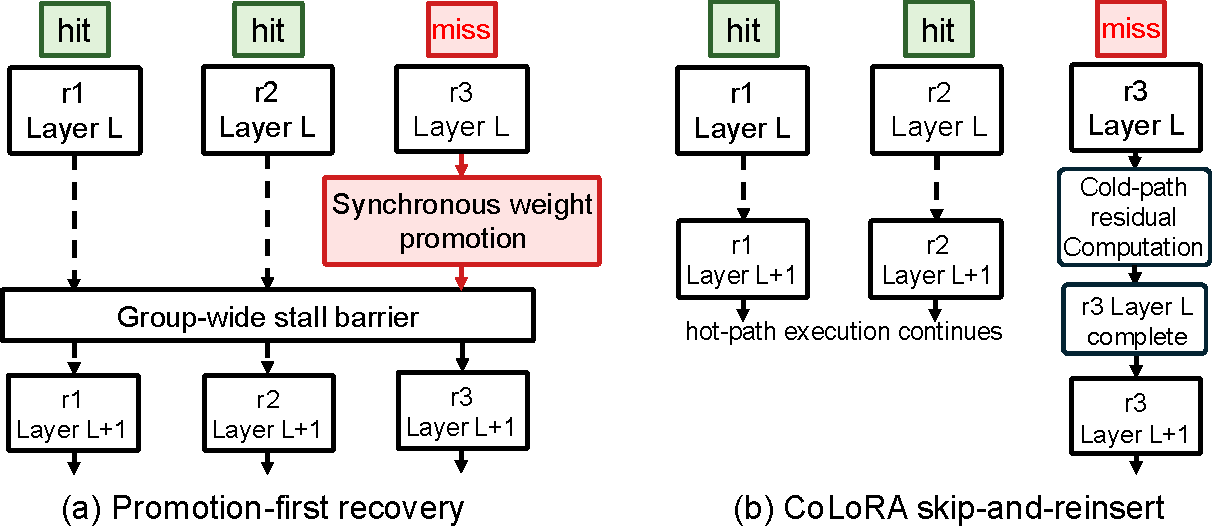
\includegraphics[width=\linewidth]{figures/skip_reinsert_scheduler.pdf}
    \caption{
    \textbf{Layer-level skip-and-reinsert scheduling.}
 Under promotion-first recovery, a cold miss can trigger synchronous weight promotion and stall the co-scheduled group. CoLoRA instead treats the miss as request-local: the faulting request leaves the hot path at layer $L$, while other GPU-ready requests continue whenever dependencies allow. After the missing residual is computed and merged at layer $L$, the request resumes at its next valid execution point, preserving per-request layer order.
    }
    \label{fig:skip-reinsert}
\end{figure}

Figure~\ref{fig:skip-reinsert} highlights the scheduler invariant. A request may be temporarily absent from hot-path layer execution, but it is never allowed to advance past an unresolved layer. Reinsertion means resuming after the request's own layer-$L$ state is complete; it does not require rejoining the same sub-batch as the requests that continued on the GPU.

\noindent\textbf{Scheduler state model.}
Each request cycles through three states: \textit{GPU-Ready}, \textit{Cold-Path}, and \textit{Awaiting Reinsertion}. The scheduler maintains separate queues for these states and a per-request layer counter. This lets requests diverge temporarily across execution phases without violating strict per-request layer order.

\noindent\textbf{Miss handling workflow.}
When a miss is detected at layer $L$, the scheduler removes the faulting request from the GPU-ready queue, stages the required activation state, and enqueues a cold-path job for the missing residual. The GPU dispatch loop can continue issuing work for remaining ready requests without introducing a foreground promotion barrier. The skipped request's device-side decode state, including KV-cache handles and layer metadata, remains valid; only the missing LoRA contribution is deferred. Once the CPU cold path returns the residual, the scheduler places the request into the reinsertion queue. After the residual is merged into the request's layer-$L$ activation state, the request is returned to the GPU-ready queue.

\noindent\textbf{Bounded cold-path concurrency.}
Decoupling miss recovery introduces a resource-management problem: too many simultaneous misses can make host execution or PCIe transfers a new queueing bottleneck. CoLoRA caps the number of in-flight cold-path jobs at $K$, tuned to available host cores and copy capacity. Excess misses are queued rather than dispatched immediately. This bound is not a correctness condition; it is a backpressure mechanism that keeps the cold path from becoming an unbounded source of latency variance. Within this bound, per-request layer order is preserved, requests may temporarily diverge to create overlap, and GPU forward progress continues whenever the GPU-ready queue is non-empty.

The scheduler does not eliminate the per-request cost of a cold miss. It changes how the cost is exposed: a miss becomes a request-local side-path recovery event rather than a batch-visible foreground weight-migration barrier. Decoupled scheduling handles the current miss, but does not by itself improve future residency or reuse. CoLoRA therefore complements it with background future-reuse policies that improve later hot-path hits without becoming prerequisites for current-token progress.

\subsection{Locality-Driven Background Optimizations}
\label{subsec:locality-background}

Execution-first recovery changes how CoLoRA serves the current miss, but not the need to manage future GPU residency under fragmented locality. Repeatedly reused cold objects should not keep paying cold-path cost, yet indiscriminate promotion would waste PCIe bandwidth and GPU memory on weakly reusable objects. CoLoRA therefore separates current-token recovery from future-reuse optimization: cold-path execution completes the present access, while deferred promotion and selective temporal predispatch operate only in the background to improve later hot-path hits.

\noindent\textbf{Deferred promotion.}
Promotion remains useful when future reuse is likely, but CoLoRA changes its role. Promotion no longer serves as the default recovery mechanism for the current miss. Instead, it becomes a background optimization whose purpose is to increase the probability that subsequent accesses execute on the GPU hot path.

When a cold-path execution is triggered, CoLoRA may asynchronously enqueue the corresponding expert--LoRA object for promotion into GPU memory. This promotion is issued off the current-token critical path and does not delay completion of the access that caused the miss. In effect, cold-path execution serves the present access, while deferred promotion improves residency for future accesses when the investment is likely to pay off.

\noindent\textbf{Reuse-aware admission.}
Deferred promotion must be selective. Otherwise, the system can spend PCIe bandwidth and GPU memory capacity on objects whose reuse is too weak to amortize promotion. CoLoRA therefore uses a reuse-aware admission policy. Let $\delta$ denote a reuse threshold. An object is admitted for asynchronous promotion only when its predicted reuse distance is within the next $\delta$ decode steps. Objects whose predicted reuse distance exceeds $\delta$ remain host-resident and continue to be served on demand through the cold path.

This policy preserves CoLoRA's execution-first semantics. Admission decisions affect future cache efficiency, not correctness or the foreground dependency chain of the current access. A wrong admission decision may reduce a later hit rate or consume bounded background bandwidth, but it does not force the current request to wait for promotion. In the current design, $\delta$ is a static hyperparameter. This keeps admission simple and makes reuse-aware promotion explicit; adaptive tuning based on runtime signals is possible but orthogonal to CoLoRA’s execution-first semantics.
%In the current design, $\delta$ is implemented as a static hyperparameter; adapting it online using observed reuse, PCIe queue depth, or device-memory pressure is left to future work.

\noindent\textbf{Selective temporal predispatch.}
The second background mechanism exploits short-horizon temporal locality in decode. Although long-horizon reuse of expert--LoRA objects can be weak under multi-tenant serving, consecutive decode tokens often preserve partial routing continuity. Our router traces show strong but layer-dependent expert-set continuity: the mean expert-set hit rate is 72.2\% overall, with early layers exceeding 95\%, middle layers dipping to 56.8\%, and late layers recovering to 87\% (Appendix~\ref{app:temporal-locality}, Figure~\ref{fig:temporal_locality_hit_rate}). This pattern suggests that short-horizon prediction can still be useful even when global cache locality is fragmented.

CoLoRA leverages this signal with selective temporal predispatch. A lightweight predictor identifies expert candidates likely to be accessed in the next few decode steps and opportunistically predispatches the corresponding host-resident weights. Predispatch is treated strictly as a background action rather than a dependency for forward progress. A request never waits for predispatch to complete: if the required object is still unavailable when accessed, execution-first cold-path recovery remains the fallback.

The purpose of predispatch is not to guarantee host-side residency at any specific cache level. Rather, it moves preparation work earlier and can reduce the service time of later cold-path invocations when predictions are correct. Incorrect predictions consume only bounded background resources and do not affect correctness or foreground progress.

Together, deferred promotion and selective temporal predispatch preserve CoLoRA's separation of responsibilities. The current access is served by the foreground path that can make immediate progress, while locality-driven mechanisms operate only in the background to improve how similar accesses are handled later.


\section{Implementation}
\label{sec:implementation}

We implement CoLoRA by extending VaLoRA~\cite{mi2025empower}. CoLoRA reuses VaLoRA's KV-cache manager, continuous batching scheduler, and token-level memory manager, and adds expert--LoRA residency lookup, cold-path residual execution, and background residency management in C++/CUDA and Python. In total, CoLoRA adds execution-first miss recovery while preserving VaLoRA's continuous-batching serving substrate for hot-path execution.

\textbf{Residency-aware dispatch.}
CoLoRA replaces adapter-centric cache entries with expert--LoRA joint objects, keyed by \texttt{(projection, layer, expert, adapter)}. A rank-$r$ joint object is charged $r$ cache slots in VaLoRA's allocator. Before each expert FFN LoRA computation, CoLoRA checks GPU residency: hits use the existing GPU LoRA path, while misses enter the CPU cold path.

\textbf{Cold-path execution and scheduling.}
The cold path computes only the missing LoRA residual; base MoE expert computation remains on the GPU. Cold-path jobs run on a bounded worker pool using vectorized AVX-512 kernels over host-resident expert--LoRA weights. Activations and residuals are transferred asynchronously through pinned staging buffers, and in-flight cold-path jobs are capped to avoid CPU or PCIe queue buildup. We extend VaLoRA's batching loop with per-request layer counters and three states: \textit{GPU-Ready}, \textit{Cold-Path}, and \textit{Awaiting Reinsertion}. On a miss at layer~$L$, only the faulting request leaves the GPU-ready batch; after its residual is returned and merged into the layer-$L$ state, the request is reinserted at its next valid layer boundary.

\textbf{Background residency management.}
Promotion, eviction, and temporal predispatch run in the background. Promotion is gated by a reuse threshold and a transfer budget, so current-token recovery never waits for promotion. Eviction uses a Chameleon-style frequency, recency, and size score~\cite{iliakopoulou2025chameleon}. The temporal predispatch uses recent per-request, per-layer routing history to issue low-priority H2D transfers only when PCIe capacity is available.


\section{Evaluation}
\label{sec:evaluation}

\subsection{Experiment Setup}
\label{subsec:setup}

\noindent {\bf Testbed and model.}
We evaluate CoLoRA on an A100-80GB server with an Intel Xeon Gold 5520+ CPU and 376~GiB host memory. Unless otherwise noted, we use a disaggregated prefill/decode deployment with one A100 for prefill and one for decode, following split-phase serving~\cite{patel2024splitwise,agrawal2023sarathi}. 

We report TPOT and output-token throughput on the decode GPU only; prompt processing runs on the prefill GPU and does not contend with decode-path latency. Each GPU connects to the host through an independent PCIe Gen4 x16 link. CPU cold-path workers are pinned to physical cores and use pinned host buffers for activation and residual transfers.

Our main evaluation uses Qwen3-VL-MoE-30B-A3B as the sparse MoE backbone, with base weights resident on the decode GPU and expert--LoRA objects stored in host memory and cached on demand. To test cross-model generality, we also evaluate Mixtral-8$\times$7B in a sensitivity study. Because its unquantized weights do not fit on a single A100-80GB, we run it with tensor parallelism degree~2, using two A100s for prefill and two for decode. For both backbones, LoRA modules are attached to expert FFN layers, and CoLoRA manages residency at expert--LoRA granularity, keyed by projection, layer, expert, and adapter identity.

%TODO[e2e-fig:second-model] Add Mixtral-8x7B as second model backbone for cross-model validation.
%TODO[e2e-fig:second-model] Consider adding larger 235B-class MoE model for scalability claim.

\noindent {\bf Baselines and variants.}
We compare three miss-recovery policies within the same VaLoRA-based runtime. All use the same expert--LoRA cache object definition and differ only in demand-miss handling. {\em S-LoRA-Expert} is our promotion-first baseline: it follows load-then-run recovery semantics~\cite{sheng2024slora}, but at expert--LoRA granularity, synchronously promoting the required object before continuing the current token. {\em CoLoRA-Min} isolates execution-first recovery by disabling deferred promotion and temporal predispatch, so GPU-resident objects use the hot path while cold objects use the CPU cold path. {\em CoLoRA-Full} adds deferred promotion and temporal predispatch. We use intermediate variants for ablation.

\noindent {\bf Workloads and datasets.}
We evaluate CoLoRA on Alibaba-trace-driven workloads and use controlled workloads to study boundary conditions. For the trace-driven workloads, we sample request arrivals and LoRA adapter IDs from Alibaba serving traces~\cite{lin2025understanding} at varying rates to fit our testbed capacity, following prior LoRA-serving trace-sampling methodology~\cite{mi2025empower}. Controlled workloads vary request arrival rate, adapter diversity, cache budget, and warmup/measurement configuration to stress high-miss regimes. In both settings, prompt and output lengths are drawn from LMSYS-CHAT-1M~\cite{zheng2023lmsyschat1m} and QMSum~\cite{zhong2021qmsum,tan2024lloco}, and expert--LoRA accesses are generated during replay by the MoE router.

\noindent {\bf Metrics.}
TODO: Revise based on the actual metrics. 
We focus on decode latency and report TPOT at P50, P90, P95, and P99, along with TTFT, end-to-end latency, request throughput, and output-token throughput. For cache-pressure analysis, we distinguish lookup-time misses from post-recovery residency: \emph{demand-key miss rate} is the fraction of expert--LoRA accesses that are non-resident when first requested, while \emph{post-recovery cache hit rate} records whether the object is resident when GPU execution occurs. This avoids making promotion-first baselines appear miss-free because they synchronously promote missing objects before execution. We also log recovery counters, including blocking promotions, CPU cold-path executions, weight H2D traffic, activation/residual transfers, queueing time, reinsertion latency, and prefetch/promotion activity. Each workload is replayed across variants with identical configurations and seeds after expert--LoRA cache-pressure calibration.

\subsection{End-to-End Performance}
\label{subsec:e2e}

\subsubsection{Real Trace Performance}
\label{subsec:real-trace}

\begin{figure}[t]
  \centering
  \vspace{-0.35em}

  \includegraphics[width=0.90\columnwidth]{figures/evaluation/e2e_scaling_shared_legend.pdf}

  \vspace{-0.45em}

  \begin{minipage}{0.485\columnwidth}
    \centering
    \small\textbf{(a) P99 TPOT}\\[-0.25em]
    \includegraphics[width=\linewidth]{figures/evaluation/e2e_scaling_p99_nolegend.pdf}
  \end{minipage}
  \hfill
  \begin{minipage}{0.485\columnwidth}
    \centering
    \small\textbf{(b) Output-token throughput}\\[-0.25em]
    \includegraphics[width=\linewidth]{figures/evaluation/e2e_scaling_throughput_nolegend.pdf}
  \end{minipage}

  \vspace{-0.20em}

  \begin{minipage}{0.96\columnwidth}
    \centering
    \small\textbf{(c) TPOT CDF at 64 adapters}\\[-0.25em]
    \includegraphics[width=\linewidth]{figures/evaluation/e2e_scaling_cdf_nolegend.pdf}
  \end{minipage}

  \vspace{-0.45em}
  \caption{
    \textbf{End-to-end scaling with adapter diversity.}
    As active adapters increase, \textsc{S-LoRA-Expert} becomes increasingly
    tail-sensitive, while CoLoRA keeps P99 TPOT nearly flat. Output-token
    throughput remains comparable across policies, and CoLoRA-Full becomes
    slightly higher at high adapter diversity by reducing foreground blocking
    promotions. The 64-adapter CDF shows similar median TPOT but sharply
    separated tails.
  }
  \label{fig:e2e-scaling}
  \vspace{-0.75em}
\end{figure}

We first evaluate how CoLoRA's tail latency scales with adapter diversity, the main axis along which expert--LoRA working sets fragment (Section~\ref{subsec:motivation}). Using the trace-derived workload described above, we vary the number of concurrently active LoRA adapters from 4 to 64 while replaying the same arrival pattern at each point. As adapter diversity increases, the number of distinct expert--LoRA joint keys grows substantially, driving the demand miss rate from 0.5\% to 17.5\% under a fixed 16~GB GPU cache budget.

Figure~\ref{fig:e2e-scaling}(a) reports P99 TPOT as a function of active adapters. \textsc{S-LoRA-Expert} becomes increasingly sensitive to adapter diversity: its P99 TPOT grows from 73.5\,ms at 4 adapters to 125.0\,ms at 64 adapters ($1.7{\times}$), with the sharpest increase between 16 and 32 adapters as foreground weight promotion becomes more exposed in the tail. In contrast, CoLoRA-Full remains nearly flat across the sweep, increasing from 66.8\,ms to 70.0\,ms ($1.05{\times}$). CoLoRA-Min, which isolates the execution-first hot/cold split, stays within 16--18\% of CoLoRA-Full from 8 adapters onward, and within 7\% at 4 adapters where misses are rare. This shows that the primary benefit comes from removing blocking promotion from foreground miss recovery; background optimization further reduces the exposed cost under higher miss pressure. The relative advantage therefore grows with adapter diversity: CoLoRA-Full is 9\% lower than \textsc{S-LoRA-Expert} at 4 adapters and 44\% lower at 64 adapters.

Figure~\ref{fig:e2e-scaling}(b) reports output-token throughput across the adapter-diversity sweep. All policies remain comparable, indicating that CoLoRA's tail-latency improvement does not come from reducing decode throughput. At low adapter diversity, throughput is nearly identical because misses are rare. At high adapter diversity, CoLoRA-Full becomes slightly higher than \textsc{S-LoRA-Expert}; at 64 adapters, throughput increases from 147.5 to 151.0~tok/s. By removing blocking foreground promotions and shifting useful weight movement to deferred background promotion, CoLoRA-Full reduces decode-path stalls while preserving GPU hot-path progress.

Figure~\ref{fig:e2e-scaling}(c) isolates the distributional effect at 64 adapters, the highest-pressure configuration in this sweep. The median TPOT is nearly identical across all policies because cache-resident objects still execute on the GPU hot path. The difference is concentrated in the tail: the P99/P50 ratio drops from $2.9{\times}$ under \textsc{S-LoRA-Expert} to $1.9{\times}$ under CoLoRA-Min and $1.6{\times}$ under CoLoRA-Full. At P95, CoLoRA-Full is 20--25\% faster than the baseline; at P99, the advantage widens to 44\%. This confirms that CoLoRA targets miss-induced tail events rather than changing the common hot-path case.


\begin{table}[t]
  \centering
  % \footnotesize
  \setlength{\tabcolsep}{3.2pt}
  \begin{tabular}{@{}lccc@{}}
    \toprule
    \textbf{Metric} & \textbf{SLE} & \textbf{C-Min} & \textbf{C-Full} \\
    \midrule
    Lookup miss rate        & 17.5\% & 17.5\% & 17.5\% \\
    Blocking promotions     & 495    & 0      & 0      \\
    CPU cold executions     & 0      & 495    & 488    \\
    Weight H2D (GB)         & 0.62   & 0.00   & 0.28   \\
    Activation D2H (GB)     & 0      & 0.002  & 0.002  \\
    Residual H2D (GB)       & 0      & 0.007  & 0.007  \\
    Cold/GPU overlap rate   & 0\%    & 30\%   & 55\%   \\
    \bottomrule
  \end{tabular}
  \caption{
    \textbf{Mechanism counters at 64 adapters.}
    SLE denotes \textsc{S-LoRA-Expert}. C-Min denotes CoLoRA-Min, and C-Full denotes CoLoRA-Full. Counters are aggregated over the same measurement window. The miss rate is measured at lookup time, before recovery. CoLoRA eliminates foreground blocking weight promotion from demand miss recovery and replaces foreground recovery with activation/residual-sized cold-path exchanges. Weight H2D under CoLoRA-Full is deferred background promotion traffic for future reuse, not foreground demand-miss recovery.
  }
  \label{tab:real-trace-mechanisms}
  \vspace{-2.7 em}
\end{table}

Table~\ref{tab:real-trace-mechanisms} explains the mechanism behind the 64-adapter result. All policies see the same 17.5\% lookup miss rate, so the latency reduction does not come from eliminating demand misses. Instead, CoLoRA changes how those misses are recovered. \textsc{S-LoRA-Expert} turns 495 misses into foreground blocking promotions and transfers 0.62\,GB of weights on the decode path. CoLoRA-Min replaces these foreground promotions one-to-one with 495 CPU cold executions, while CoLoRA-Full eliminates foreground blocking promotions and serves 488 cold-path executions, with the remaining weight movement shifted to background promotion for future reuse. In both CoLoRA variants, demand recovery exchanges only activation/residual-sized state on the foreground path. CoLoRA-Full further overlaps 55\% of cold-path recovery time with GPU hot-path execution; its 0.28\,GB of weight H2D traffic comes from deferred background promotion, not foreground miss recovery. 

Taken together, these results show that CoLoRA improves tail latency by changing how misses are recovered, not by eliminating misses. Execution-first recovery is effective because it treats cold misses as bounded heterogeneous execution events whose exposed cost grows more slowly with adapter diversity than synchronous weight promotion.

\subsubsection{Controlled Pressure Performance}
\label{subsec:controlled-pressure}

\begin{figure}[t]
  \centering
  \includegraphics[width=0.90\columnwidth]{figures/evaluation/e2e_scaling_shared_legend.pdf}

  \vspace{-0.45em}

  \begin{subfigure}[t]{0.48\columnwidth}
    \centering
    \small\textbf{(a) P99 vs. cache budget}\\[-0.15em]
    \includegraphics[width=\linewidth]{figures/evaluation/controlled_p99_vs_cache.pdf}
  \end{subfigure}
  \hfill
  \begin{subfigure}[t]{0.48\columnwidth}
    \centering
    \small\textbf{(b) Tail under high pressure}\\[-0.15em]
    \includegraphics[width=\linewidth]{figures/evaluation/controlled_tail_percentiles.pdf}
  \end{subfigure}

  \vspace{-0.45em}
  \caption{\textbf{Controlled-pressure performance.}
  (a) Under tight cache budgets, promotion-first recovery exposes weight-transfer
  stalls, while CoLoRA reduces P99 TPOT by serving cold misses through execution-first
  recovery. As the cache budget increases and objects become resident, all policies converge.
  (b) At the tightest budget, all policies have similar median TPOT, but CoLoRA sharply
  compresses the tail: the P99/P50 ratio drops from $9.0{\times}$ under load-then-run to
  $4.4{\times}$ under CoLoRA-Full.}
  \label{fig:controlled-pressure}
  \vspace{-0.75em}
\end{figure}

To isolate CoLoRA's miss-recovery mechanism from production-trace skew, we next evaluate a controlled-pressure workload that stresses the high-miss regime identified in Section~\ref{sec:background}. This workload is a stress setting rather than a direct production model: it creates frequent expert--LoRA misses while preserving a stable GPU hot set, allowing us to study when execution-first recovery helps and when its advantage naturally diminishes. We use 4 LoRA adapters, which can all fit into the 16GB GPU cache at the largest budget.

Figure~\ref{fig:controlled-pressure}(a) shows P99 TPOT as a function of cache budget. Under tight budgets, where hot-set coverage remains limited, CoLoRA-Full reduces P99 TPOT by 51--55\% over \textsc{S-LoRA-Expert}. CoLoRA-Min, which disables deferred promotion and temporal predispatch, captures 64--67\% of this improvement, confirming that the main benefit comes from replacing foreground promotion with execution-first cold-path recovery. As cache capacity increases and demand misses become rare, the gap narrows. At the largest budget, where the working set nearly fits in GPU memory, all policies begin to converge because miss recovery is no longer the main source of tail latency.

Figure~\ref{fig:controlled-pressure}(b) examines the tightest-budget case in more detail. \textsc{S-LoRA-Expert} exhibits a long latency tail because weight promotion is exposed on the decode critical path. CoLoRA-Full compresses this tail: the P99/P50 ratio drops from $9.0{\times}$ to $4.4{\times}$, and the fraction of tokens exceeding 100\,ms falls from 52\% to 8\%. Mechanism counters confirm that the improvement comes from replacing foreground blocking weight promotion with CPU cold-path recovery, reducing critical-path transfer volume from 15.5\,GB to 0.19\,GB.

These controlled-pressure results show both the strength and the boundary of CoLoRA's design. When misses are frequent and near-term reuse is weak, execution-first recovery prevents cold misses from becoming dominant promotion stalls. When the working set nearly fits in GPU memory, the policies converge because miss recovery is no longer the main source of latency variance.

\subsection{Single-Miss Recovery Microbenchmark}
\label{subsec:microbenchmark}

\begin{figure}[t]
  \centering
  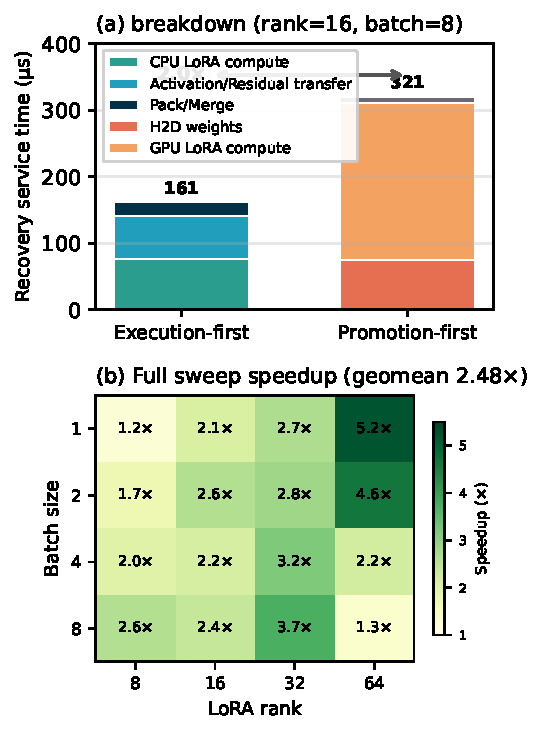
\includegraphics[width=\linewidth]{figures/fig_cold_recovery_singlecol.pdf}
  \caption{
  Single-miss recovery at one MoE layer.
  (a) Standalone recovery-time breakdown for one cold expert--LoRA
  object at rank 16 and decode batch size 8.
  Thin gray segments denote object admission for promotion-first and
  activation packing/result merging for execution-first.
  Promotion-first pays full-object H2D transfer before GPU LoRA execution,
  while execution-first exchanges activation/residual-sized state and
  computes the missing residual on the CPU.
  (b) Speedup of execution-first over promotion-first across LoRA ranks and
  decode batch sizes.
  }
  \label{fig:microbreakdown}
\end{figure}

We next isolate the local cost of recovering one GPU-cold expert--LoRA object at a single MoE layer. This microbenchmark evaluates the cost model in Section~\ref{subsec:feasibility} before scheduler overlap is introduced. A promotion-first miss must restore GPU residency by transferring the full expert--LoRA object before the current token can resume. In contrast, execution-first recovery completes the current access by sending activation state to the host, computing the missing LoRA residual from host-resident weights, and returning only the residual to the GPU. The goal is not to show that CPU execution is generally faster than GPU execution, but to test whether replacing full-object migration with activation/residual-sized exchange reduces the synchronous cost of one cold recovery.

To keep the measurement local, we disable cache replacement, request scheduling, queueing, deferred promotion, temporal predispatching, and cross-request overlap. The reported time therefore measures the standalone service time of the recovery path, not the end-to-end latency exposed by the full runtime. Here, decode batch size denotes the number of activations served by the isolated recovery path for the same missing expert--LoRA object. Promotion-first transfers the missing object to GPU memory and then computes the LoRA residual on the GPU. Execution-first transfers the current activations to the host, computes the residual on the CPU, and returns the residuals to the GPU.

We instrument the components on both recovery paths. For promotion-first, we report cache-admission overhead, H2D expert--LoRA weight transfer, and GPU LoRA computation. For execution-first, we report activation packing, D2H activation transfer, CPU residual computation, H2D residual transfer, and merge. We sweep LoRA rank $\{8,16,32,64\}$ and decode batch size $\{1,2,4,8\}$, covering the small-batch decode regime where per-token stalls are most visible.

Figure~\ref{fig:microbreakdown} reports the standalone service time of one cold recovery. In the representative rank-16, batch-8 configuration, promotion-first takes 321~$\mu$s, while execution-first takes 161~$\mu$s. The breakdown shows that the gap comes primarily from the critical-path payload: promotion-first waits for full expert--LoRA weight transfer before execution can resume, whereas execution-first avoids this transfer and instead pays CPU residual computation plus small activation/residual transfers.

Across the sweep, execution-first is faster in all 16 configurations, with speedups from 1.2$\times$ to 5.2$\times$ and a 2.45$\times$ geometric mean. The speedups are not monotonic in either rank or batch size because the two recovery paths scale with different quantities. Promotion-first is dominated by full-object transfer, which grows with LoRA rank and is largely insensitive to decode batch size. Execution-first instead scales with CPU residual computation and staging overhead, which grow with both rank and batch size. As a result, execution-first has the largest advantage when weight movement dominates, while the gap narrows when CPU-side residual computation becomes the larger term.

These results validate the predicted payload asymmetry at the single-miss level. For a cold expert--LoRA object, the critical cost is not only where the residual is computed, but what state must be moved before the current decode step can proceed. In the full runtime, this local service-time advantage becomes an end-to-end tail-latency benefit when demand misses are frequent enough and when the scheduler can overlap cold-path work with GPU-ready execution. Thus, the 2.45$\times$ standalone speedup helps explain the P99 reduction observed in Section~\ref{subsec:real-trace}, but should be interpreted together with the measured demand miss rate and cold/GPU overlap. When reuse is strong enough to amortize promotion, or when CPU residual computation dominates, promotion-first can remain competitive.

\subsection{Ablation Study}
\label{subsec:ablation}

\noindent {\bf Incremental ablation.} We decompose CoLoRA-Full's improvement using an ordered build-up of its mechanisms. Figure~\ref{fig:ablation-promotion} compares four miss-recovery policies at 64 adapters. We use this controlled setting because it creates enough demand misses to expose differences among recovery policies while keeping the workload fixed across variants. Starting from \textsc{S-LoRA-Expert} (125.0~ms P99 TPOT), asynchronous promotion peels off the faulting request on a miss and reinserts it after H2D transfer completes, without CPU cold-path execution. This reduces P99 to 109.0~ms, a 12.8\% improvement relative to \textsc{S-LoRA-Expert}. The gain is modest because the faulting request still waits for the full expert--LoRA object to be transferred before it can resume, and reinsertion itself introduces overhead.

Adding CPU cold-path execution on top of asynchronous promotion (CoLoRA-Min) further reduces P99 to 82.5~ms, a 24.3\% improvement over asynchronous promotion. This is the largest incremental gain because foreground recovery replaces full-object weight movement with activation/residual-sized exchanges and host-side residual computation. Finally, adding deferred promotion and temporal predispatch (CoLoRA-Full) reduces P99 to 70.0~ms, a further 15.2\% improvement. Thus, in this ordered build-up, the CPU cold path provides the largest incremental gain, while asynchronous promotion and background reuse policies provide complementary improvements. Together, the mechanisms explain CoLoRA-Full's 44.0\% P99 reduction over \textsc{S-LoRA-Expert}.

\noindent {\bf Overlap effectiveness.} We next isolate whether the scheduler can overlap recovery work with GPU-ready execution while holding each recovery policy fixed. In the no-overlap variant, a request that enters promotion or CPU cold-path recovery prevents the decode step from advancing until the recovery result is available; all cache decisions and recovery mechanisms are unchanged. Disabling this overlap makes miss recovery synchronous with respect to the decode step. P99 rises from 82.5 to 106.0~ms for CoLoRA-Min and from 70.0 to 93.0~ms for CoLoRA-Full; throughput drops from 148.0 to 135.5~tok/s and from 147.5 to 134.0~tok/s, respectively. Thus, overlap reduces P99 by 22--25\% relative to the no-overlap variants by hiding recovery work behind GPU hot-path execution. This validates the scheduler design in Section~\ref{subsec:scheduler}: skip-and-reinsert is necessary for converting cold-path service-time reduction into end-to-end tail-latency reduction.

\noindent {\bf Reinsertion overhead.} The overlap benefit above comes from peeling off faulting requests and later reinserting them, so we also quantify the cost of this reinsertion path. We measure reinsertion latency from cold-path completion callback to the request becoming eligible for its next GPU execution point, including callback scheduling, state merge, and batch synchronization. Across the controlled-pressure runs, this cost is 8.8--10.2~ms per token that triggers cold-path recovery at P99, about one-tenth of the corresponding P99 TPOT. The cost remains stable across cache budgets because the amount of work per reinsertion is fixed once a miss occurs; cache capacity changes how often reinsertion happens, not the cost of handling one completed cold-path result.

\begin{figure}[t]
  \centering
  \includegraphics[width=0.85\columnwidth]{figures/evaluation/ablation_promotion.pdf}
  \caption{
    \textbf{Incremental ablation at 64 adapters.}
    Starting from \textsc{S-LoRA-Expert}, asynchronous promotion,
    CPU cold-path execution, and background reuse policies reduce
    P99 TPOT from 125.0 to 70.0~ms. The largest incremental gain
    comes from CPU cold-path execution.
  }
  \label{fig:ablation-promotion}
\end{figure}

\subsection{Sensitivity Analysis}
\label{subsec:sensitivity}

We evaluate CoLoRA's sensitivity to deployment and workload parameters beyond the primary adapter-count sweep in Section~\ref{subsec:real-trace}. The goal is to characterize the operating envelope of execution-first recovery: how much CPU capacity it needs, when fragmented access makes it most beneficial, whether the benefit generalizes to another MoE backbone, and how the system behaves under an all-cold stress regime.

\begin{figure*}[t]
  \centering
  \includegraphics[width=\textwidth]{figures/evaluation/fig_sensitivity.pdf}
  \caption{
    \textbf{Sensitivity analysis.}
    (a) CPU worker scaling shows that cold-path queueing drops sharply up to 4 workers and then saturates.
    (b) Popularity-skew sensitivity shows that CoLoRA's advantage is largest under flat, fragmented access.
    (c) Cross-model evaluation on Mixtral-8$\times$7B tests whether execution-first recovery generalizes beyond the main Qwen MoE backbone.
    (d) The all-cold stress regime shows that CoLoRA degrades more gracefully when caching provides little reuse.
  }
  \label{fig:sensitivity}
\end{figure*}

\paragraph{CPU worker scaling.}
Figure~\ref{fig:sensitivity}(a) sweeps the number of CPU cold-path workers from 1 to 8. With a single worker, cold-path execution becomes queue-limited: the maximum queue depth reaches 365 and P99 TPOT rises to 113~ms. Adding workers quickly reduces this bottleneck. Two workers reduce P99 TPOT to 84.8~ms and queue depth to 122; four workers further reduce them to 77.0~ms and 45; eight workers provide only a smaller additional gain, reaching 73.5~ms and 16. This diminishing return indicates that the cold path is no longer CPU-queue dominated beyond 4 workers; the remaining exposed latency comes mainly from transfer, merge, and reinsertion overheads. Thus, CoLoRA does not require a large host allocation: a modest worker pool is sufficient to keep cold-path recovery bounded for this workload.

\paragraph{Popularity skew.}
Figure~\ref{fig:sensitivity}(b) varies the Zipf skew parameter of adapter access from uniform ($\alpha=0.0$) to highly skewed ($\alpha=2.0$). Increasing skew concentrates requests on fewer adapters, reduces the effective expert--LoRA working set, and improves all policies. CoLoRA's benefit is therefore largest in the harder low-locality regime. Under uniform access, \textsc{S-LoRA-Expert} reaches 180.0~ms P99 TPOT, while CoLoRA-Full reaches 76.5~ms, a 103.5~ms gap. At $\alpha=2.0$, the gap narrows to 20.5~ms (90.0 vs.\ 69.5~ms), because caching alone becomes more effective. This trend confirms the intended operating point of CoLoRA: execution-first recovery is most valuable when access is fragmented enough that misses remain unavoidable.

\paragraph{Cross-model generality.}
Figure~\ref{fig:sensitivity}(c) evaluates CoLoRA on Mixtral-8$\times$7B to test whether execution-first recovery depends on the main Qwen MoE backbone. Mixtral differs in model architecture, expert dimensions, routing behavior, and deployment shape; because its unquantized weights do not fit on a single A100-80GB, we run it with tensor parallelism degree 2 for both prefill and decode. We keep the same expert--LoRA residency abstraction and compare the same recovery policies. CoLoRA-Full reduces P99 TPOT from XX~ms to XX~ms over \textsc{S-LoRA-Expert}, while maintaining output-token throughput within XX\%. CoLoRA-Min already captures most of the reduction, showing that the execution-first cold path remains effective; CoLoRA-Full adds a smaller additional gain through deferred promotion and temporal predispatch. These results indicate that CoLoRA's benefit comes from the recovery abstraction rather than a Qwen-specific routing artifact.

\paragraph{All-cold stress regime.}
Figure~\ref{fig:sensitivity}(d) evaluates an all-cold stress regime where the demand miss rate exceeds 99\%, modeling a burst of requests for previously unseen adapters. This is not intended to represent steady-state production behavior; instead, it tests whether the system fails abruptly when caching provides almost no reuse. \textsc{S-LoRA-Expert} degrades sharply because nearly every token waits for synchronous weight promotion, reaching 820~ms P99 TPOT and 26~tok/s. CoLoRA-Min and CoLoRA-Full remain functional: P99 TPOT drops to 280~ms and 235~ms, respectively, while throughput increases to 38--42~tok/s. This behavior shows that execution-first recovery provides a bounded fallback even when future reuse is weak, and that the CPU cold path does not become an immediate throughput collapse point under extreme miss pressure.

\section{Related Work}
\label{sec:related}

\paragraph{LoRA and multi-tenant adapter serving.}
LoRA introduced low-rank adaptation as a parameter-efficient way to specialize a shared foundation model with a small number of task-specific parameters \cite{hu2022lora}. Since then, a substantial body of work has studied efficient serving of many concurrent LoRA tenants, including heterogeneous batching, adapter paging, CPU-assisted loading, and SLO-aware scheduling \cite{chen2024punica,sheng2024slora,wu2024dlora,li2025toppings,bruel2024compress}. These systems form the closest prior art on the adaptation axis. However, they primarily target dense backbones, where the active adaptation state is naturally organized around adapters. In CoLoRA's setting, the base model is sparse and each decode step touches only the LoRA states associated with the routed experts for the current token. The relevant unit of access is therefore not an adapter alone, but an expert--LoRA joint object.

\paragraph{Sparse MoE models and serving.}
Sparse MoE architectures activate only a small subset of experts per token, making routing locality central to efficient inference \cite{shazeer2017outrageously,fedus2022switch,jiang2024mixtral,zhu2024deepseek}. Correspondingly, recent MoE-serving systems study expert placement, offloading, caching, and CPU/GPU co-execution under memory pressure \cite{xue2024moe,kamahori2024fiddler,yu2025fmoe,zhong2025hybrimoe}. These works are directly relevant on the sparsity axis, but they reason primarily at expert granularity. CoLoRA addresses a different regime in which expert routing and tenant-specific adaptation interact, fragmenting reuse across a much larger space of expert--LoRA combinations. This difference is especially consequential during decode, where even infrequent cold accesses can surface directly on the per-token critical path and disproportionately affect tail latency.

\paragraph{LLM serving runtimes and hierarchical memory management.}
A complementary line of work studies the runtime substrate for efficient LLM inference, including iteration-level scheduling, continuous batching, KV-cache management, prefill/decode separation, and hierarchical use of host and device memory \cite{yu2022orca,kwon2023efficient,agrawal2023sarathi,patel2024splitwise,aminabadi2022deepspeed,sheng2023flexgen,na2025flexinfer}. CoLoRA builds on this systems context, but differs in how it handles cold weights on the decode path. Prior systems typically treat a miss as a promotion problem: weights are restored to accelerator memory before normal execution proceeds. CoLoRA instead targets cache-pressured multi-LoRA MoE decode, where many misses have weak near-term reuse and synchronous promotion can become a blocking synchronization point. In this sense, prior work has separately advanced adapter-centric LoRA serving, expert-centric MoE serving, and high-performance LLM runtime design, while CoLoRA combines these perspectives for a setting that none of them directly addresses: multi-tenant LoRA serving on sparse MoE backbones under decode-time cache pressure. Its central distinction is to make the expert--LoRA joint object the unit of control and to decouple miss recovery for the current token from residency restoration for future tokens.


\section{Conclusion}

Across trace-driven and end-to-end evaluations, CoLoRA shows that execution-first cold-miss handling improves the robustness of multi-LoRA MoE decode serving under realistic cache pressure. By removing blocking promotion from the critical path of GPU-cold misses, CoLoRA reduces tail-latency inflation while preserving efficient GPU execution for hot objects and base-model computation. 

% \section{Conclusion}
\clearpage
\bibliographystyle{plain}
\bibliography{CoLoRA-reference}

\clearpage
\appendix
\section{Per-Layer Temporal Routing Locality}
\label{app:temporal-locality}

Figure~\ref{fig:temporal_locality_hit_rate} reports the per-layer consecutive-token routing locality measured from the Qwen3--VL--MoE router on the ShareGPT--V3 trace. For each request and MoE layer, we compare the routed expert set at decode step $t$ against the previous decode step $t-1$ using the hit-rate metric $|E(L,t) \cap E(L,t-1)| / |E(L,t)|$. The resulting curve is distinctly U-shaped: early layers show very high temporal continuity, middle layers are weaker, and late layers recover. This observation motivates temporal predispatch as a useful but non-uniform optimization across depth.

\begin{figure}[t]
  \centering
  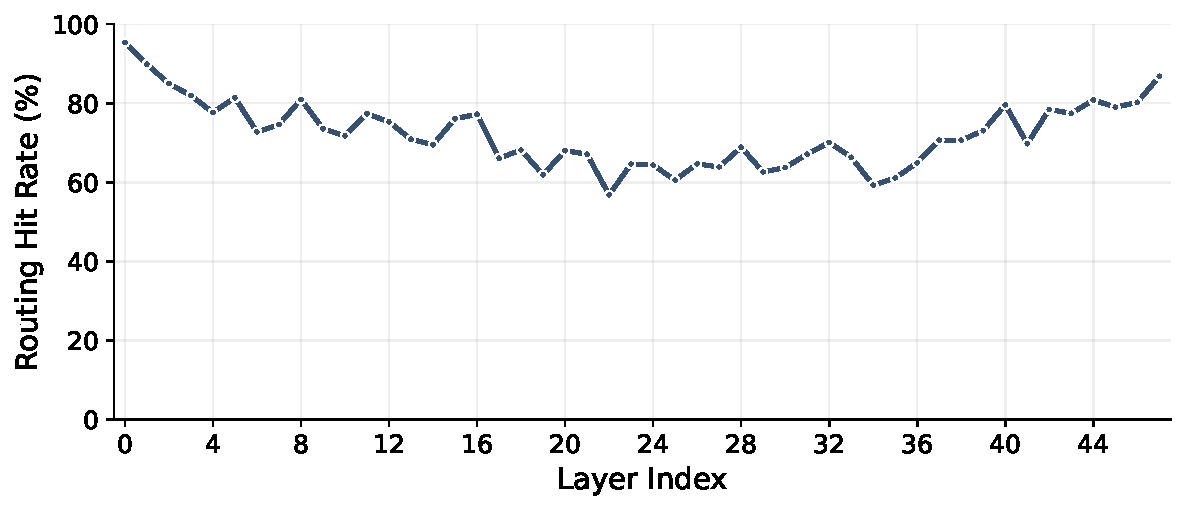
\includegraphics[width=\columnwidth]{figures/motivation/temporal_locality_hit_rate.pdf}
  \caption{
  Per-layer consecutive-token routing locality during decode.
  The plotted quantity is the mean expert-set hit rate $|E(L,t) \cap E(L,t-1)| / |E(L,t)|$.
  The curve is U-shaped: early and late layers exhibit stronger temporal continuity, while middle layers are weaker.
  This pattern supports an opportunistic, potentially layer-selective temporal predispatch policy rather than a uniform always-on rule.
  }
  \label{fig:temporal_locality_hit_rate}
\end{figure}


\end{document}
\endinput
%%
%% End of file `sample-sigconf.tex'.

